\section{Schwingung eines einzelnen Pendels}




\begin{figure}[h!]
	\centering
	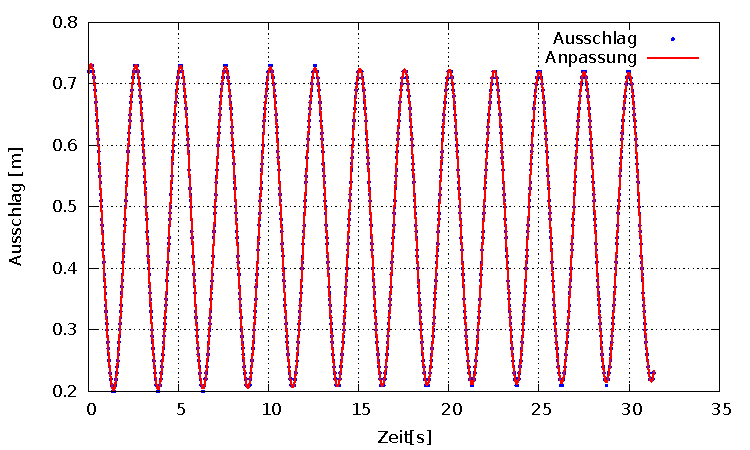
\includegraphics[width=0.7\linewidth]{Auswertung/einfach/einzelnesPendel.pdf}
	\caption{einzelnes Pendel....}
	\label{fig:einzelnespendel}
\end{figure}




\begin{align*}
	a               &= \SI{ 0.264874        \pm 0.0002243}{m}   \\
	\rho             &=\SI{ 0.00177972      \pm 4.733e-005 }{\per s} \\
	\omega            &= \SI{2.52453         \pm 4.857e-005}{\per s}  \\
	\varphi            &= 1.25363         \pm 0.0008653    \\
	c               &=\SI{ 0.466706        \pm 7.91e-005}{m}    \\
	\end{align*}